% --------------------------------------------------------------------------
% Version 3.0
% This template is available on the sites:
% https://www.overleaf.com/read/rpkkfchcnbsc
% https://www.overleaf.com/latex/templates/itmo-beamer-theme/fpttrgnmqwsb
% https://github.com/AlexZabashta/ITMO-Beamer-theme
% --------------------------------------------------------------------------

\documentclass[aspectratio=169]{beamer}
\usepackage{ITMOtheme}

% \usepackage[czech]{babel}

% Use this package to automatically format references.
% \usepackage[style=mla]{biblatex}
% \addbibresource{references.bib}

% \titlegraphic{\includegraphics[width=0.2\textwidth]{itmo/logo_basic_english_white.pdf}}

% use \title[short title]{full title}
\title[PredictionAndVisualization]{Prediction and visualization of cryptic binding regions}

% \subtitle[CryptoShow]{CryptoShow}

\author[Polak L.]{Lukáš Polák}

\institute[CUNI]{Faculty of Mathematics and Physics, Charles University}

\where{Prague}
\date{September 9, 2025}

\subject{bioinformatics}
\keywords{bioinformatics, machine learning, protein, binding sites}

\begin{document}

% [plain] - modifier to create a blank slide (without bottom bar).
% Ideal for creating the first (title) and last slide with a polygonal background,
% or for transitional slides between chapters or slides with a table of contents.

% \titlepage - command for automatic generation of title slide content.

\begin{frame}[plain]
  \titlepage
\end{frame}

% You can use custom title, if you want.
% Or you can you modify the .sty file.

% \begin{frame}[plain]
%     \itmobackgroundsnakes{
%     \vfill
%         \includegraphics[width=0.2\textwidth]{itmo/logo_basic_english_white.pdf}
%     \vfill
%         \usebeamerfont{title}{  \inserttitle\par}
%     \vfill
%         Custom title slide
%     \vfill
%         \insertauthor\par
%     \vfill
%         \insertplace  \;  \insertdate
% }
% \end{frame}

% Avoid making a table of contents in short presentations.
% Transitions between chapters are best done manually.

\AtBeginSection[]
{
  \begin{frame}[plain]
    \frametitle{Outline}
    \tableofcontents[currentsection]
  \end{frame}
}

% \begin{frame}{Footcite and Footnote}

%   Example of footnote \footnote{For example, it can be used for citation}.

% \end{frame}

\section{Introduction to Bioinformatics}

\subsection{Proteins, Amino Acids, and Protein Structures}

\begin{frame}
  \frametitle{Proteins, Amino Acids, and Protein Structures}

  \begin{itemize}
    \item \textbf{Proteins}: essential biomolecules, diverse functions
    \item Composed of \textbf{amino acid (residue)} chains
    \item \textbf{Primary structure}: amino acid sequence
    \item \textbf{Tertiary structure}: 3D folding, functional form
  \end{itemize}

\end{frame}

\subsection{Binding Sites}

\begin{frame}
  \frametitle{Binding Sites}

  \begin{itemize}
    \item \textbf{Binding sites}: regions on proteins where ligands (e.g., substrates, inhibitors) bind
    \item \textbf{Cryptic binding sites}: hidden or transient sites, not apparent in static structures
    \item \textbf{Apo/Holo conformations}: different states of a protein (apo: unbound, holo: bound)
  \end{itemize}

  \begin{itemize}
    \item Crucial for \textbf{protein function}, regulation, and interaction with other molecules
    \item Essential for \textbf{drug design} and discovery
  \end{itemize}

\end{frame}

\subsection{CryptoBench}

\begin{frame}
  \frametitle{Cryptic Binding Residues Prediction: CryptoBench}
  \begin{itemize}
    \item A benchmark dataset developed at FMP CUNI for evaluating cryptic binding site prediction methods
    \item Provides a diverse set of protein structures
    \item Includes a model for predicting individual cryptic binding \textbf{residues} (not sites)
  \end{itemize}

\end{frame}

\section{Methodology}
\subsection{Objectives}

\begin{frame}
  \frametitle{Objectives}
  \begin{block}{Clustering}
    Cluster \textbf{residue-level} cryptic predictions (CryptoBench) into contiguous \textbf{cryptic binding sites}.
  \end{block}

  \begin{block}{Software (CryptoShow)}
    Build a client–server web app to submit structures, run residue predictions, cluster them into sites, and visualize results. Additionally, provide animations using AHoJ\footnote{AHoJ is a tool developed at FMP CUNI for finding apo-holo protein pair analogs.}.
  \end{block}
\end{frame}

\subsection{Pipeline}

\begin{frame}
  \frametitle{Data Processing Pipeline}

  \begin{figure}
    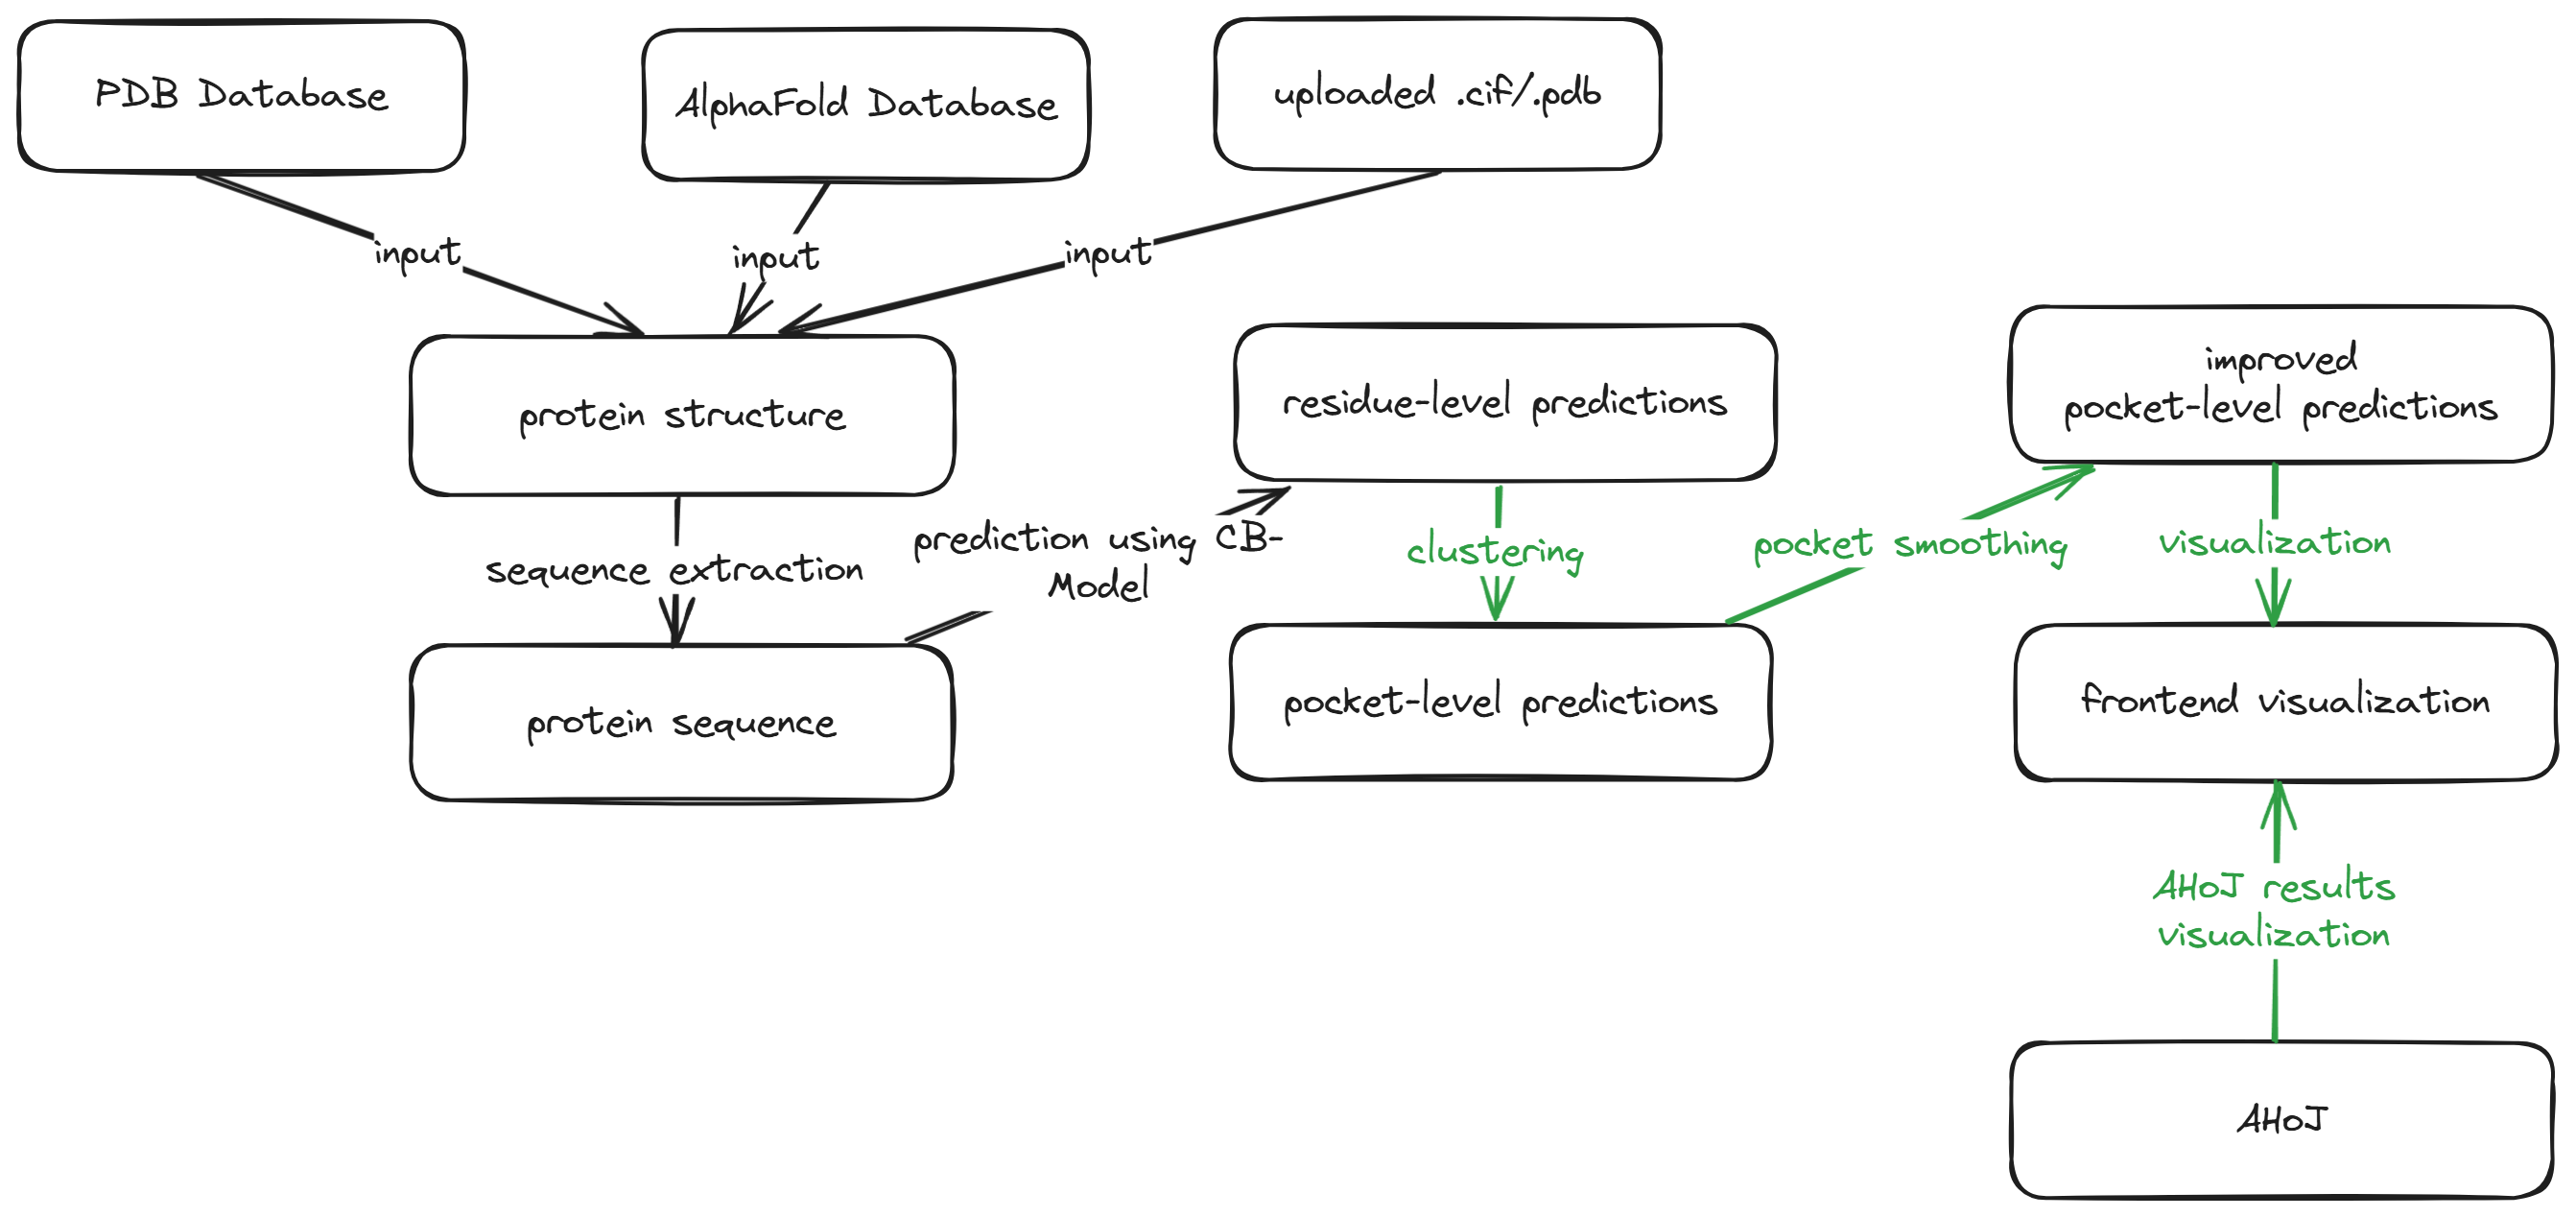
\includegraphics[width=\textwidth]{fig/pipeline.png}
    \caption{Data processing pipeline. \textcolor{ITMOdarkgreen}{Green arrows} indicate newly introduced techniques.}
  \end{figure}

\end{frame}

\subsection{Clustering}

\begin{frame}
  \frametitle{Clustering}

  \begin{columns}
    \begin{column}{0.5\textwidth}
      \textbf{Approach 1}
      \begin{itemize}
        \item DBSCAN algorithm
        \item Cluster residues within 5 \AA
        \item Based purely on sequence information
      \end{itemize}
    \end{column}
    \begin{column}{0.5\textwidth}
      \textbf{Approach 2}
      \begin{itemize}
        \item DBSCAN algorithm + smoothing model
        \item Improve clustering by adding spatial information
      \end{itemize}
    \end{column}
  \end{columns}

\end{frame}

\subsection{Evaluation}

\begin{frame}
  \frametitle{Evaluation on the CryptoBench dataset: Approach 1}

  "Simple" clustering is not enough\dots

  \begin{figure}
    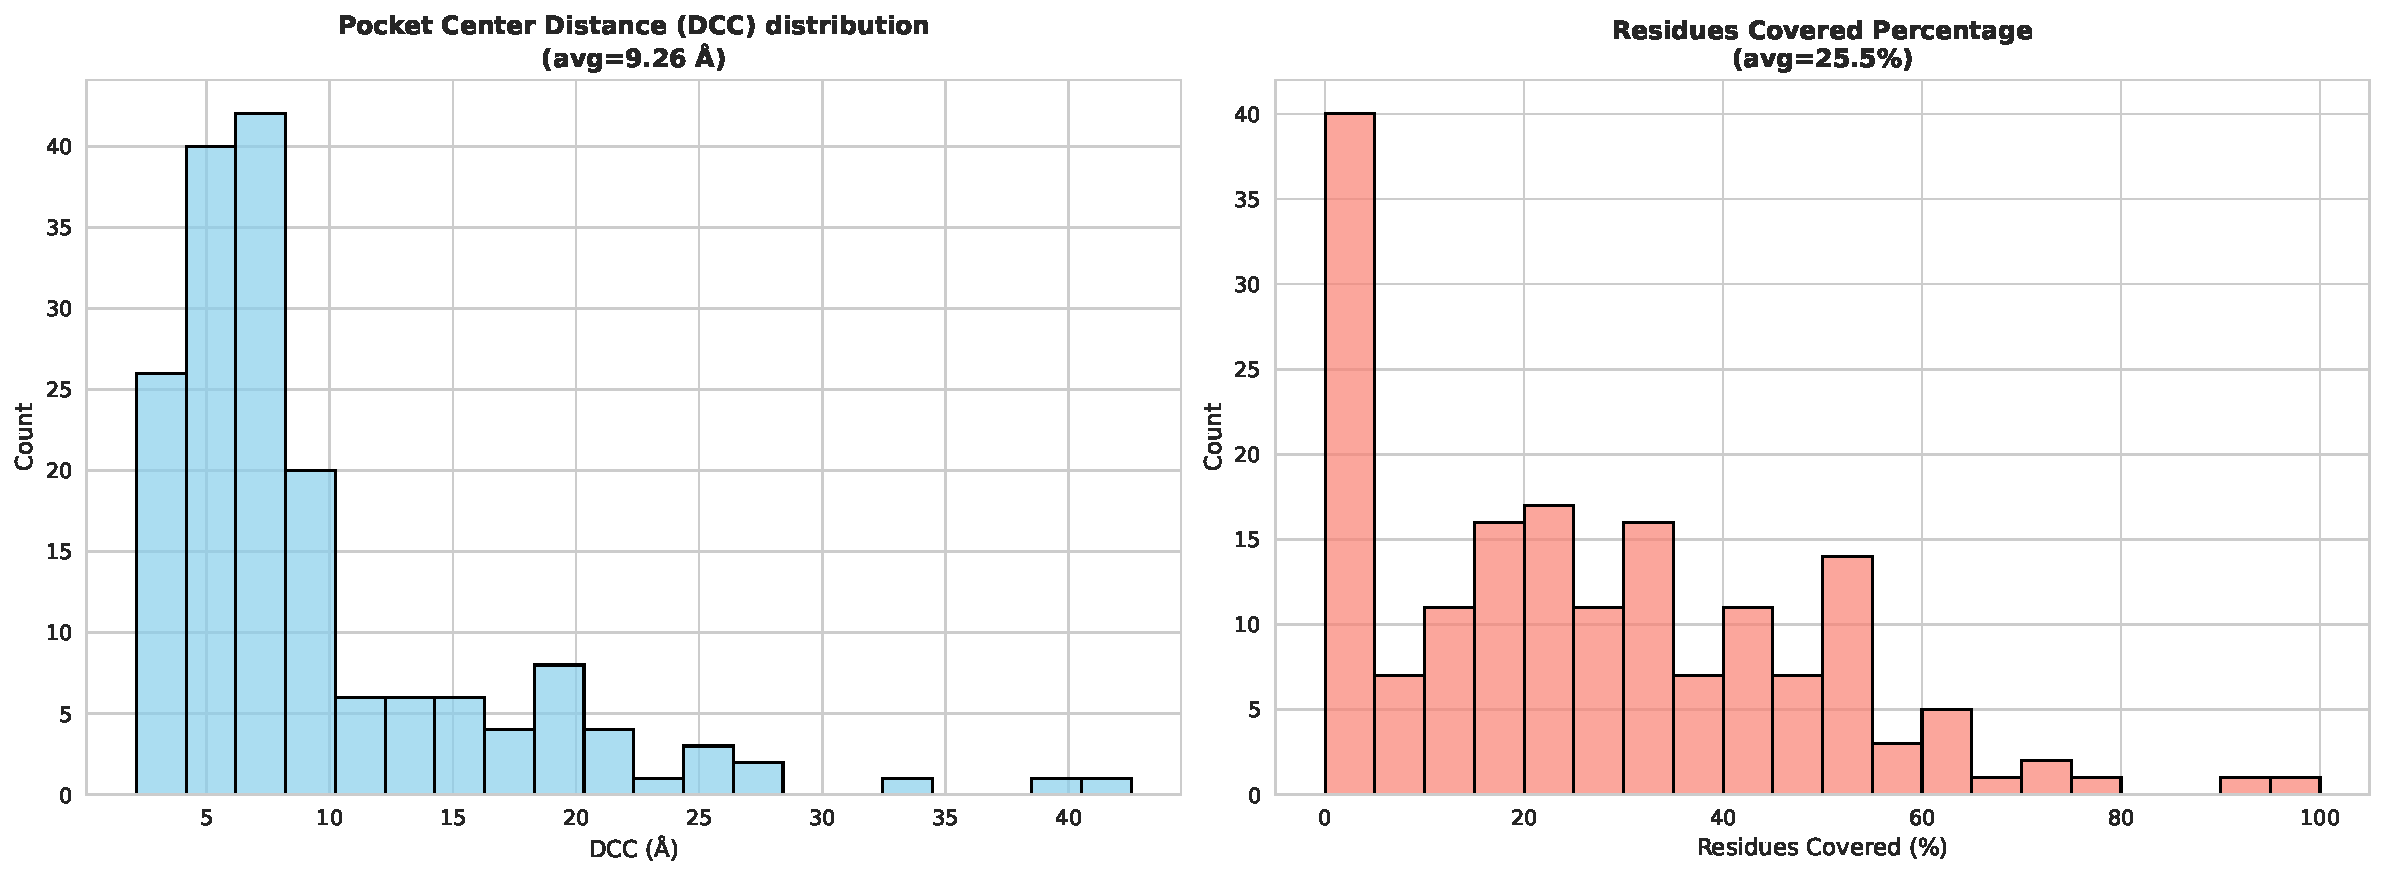
\includegraphics[width=\textwidth]{fig/non-smoothened-1.pdf}
  \end{figure}
\end{frame}

\begin{frame}
  \frametitle{Approach 2: Smoothing Model Training}

  Let's train another model!

  \begin{figure}
    \centering
    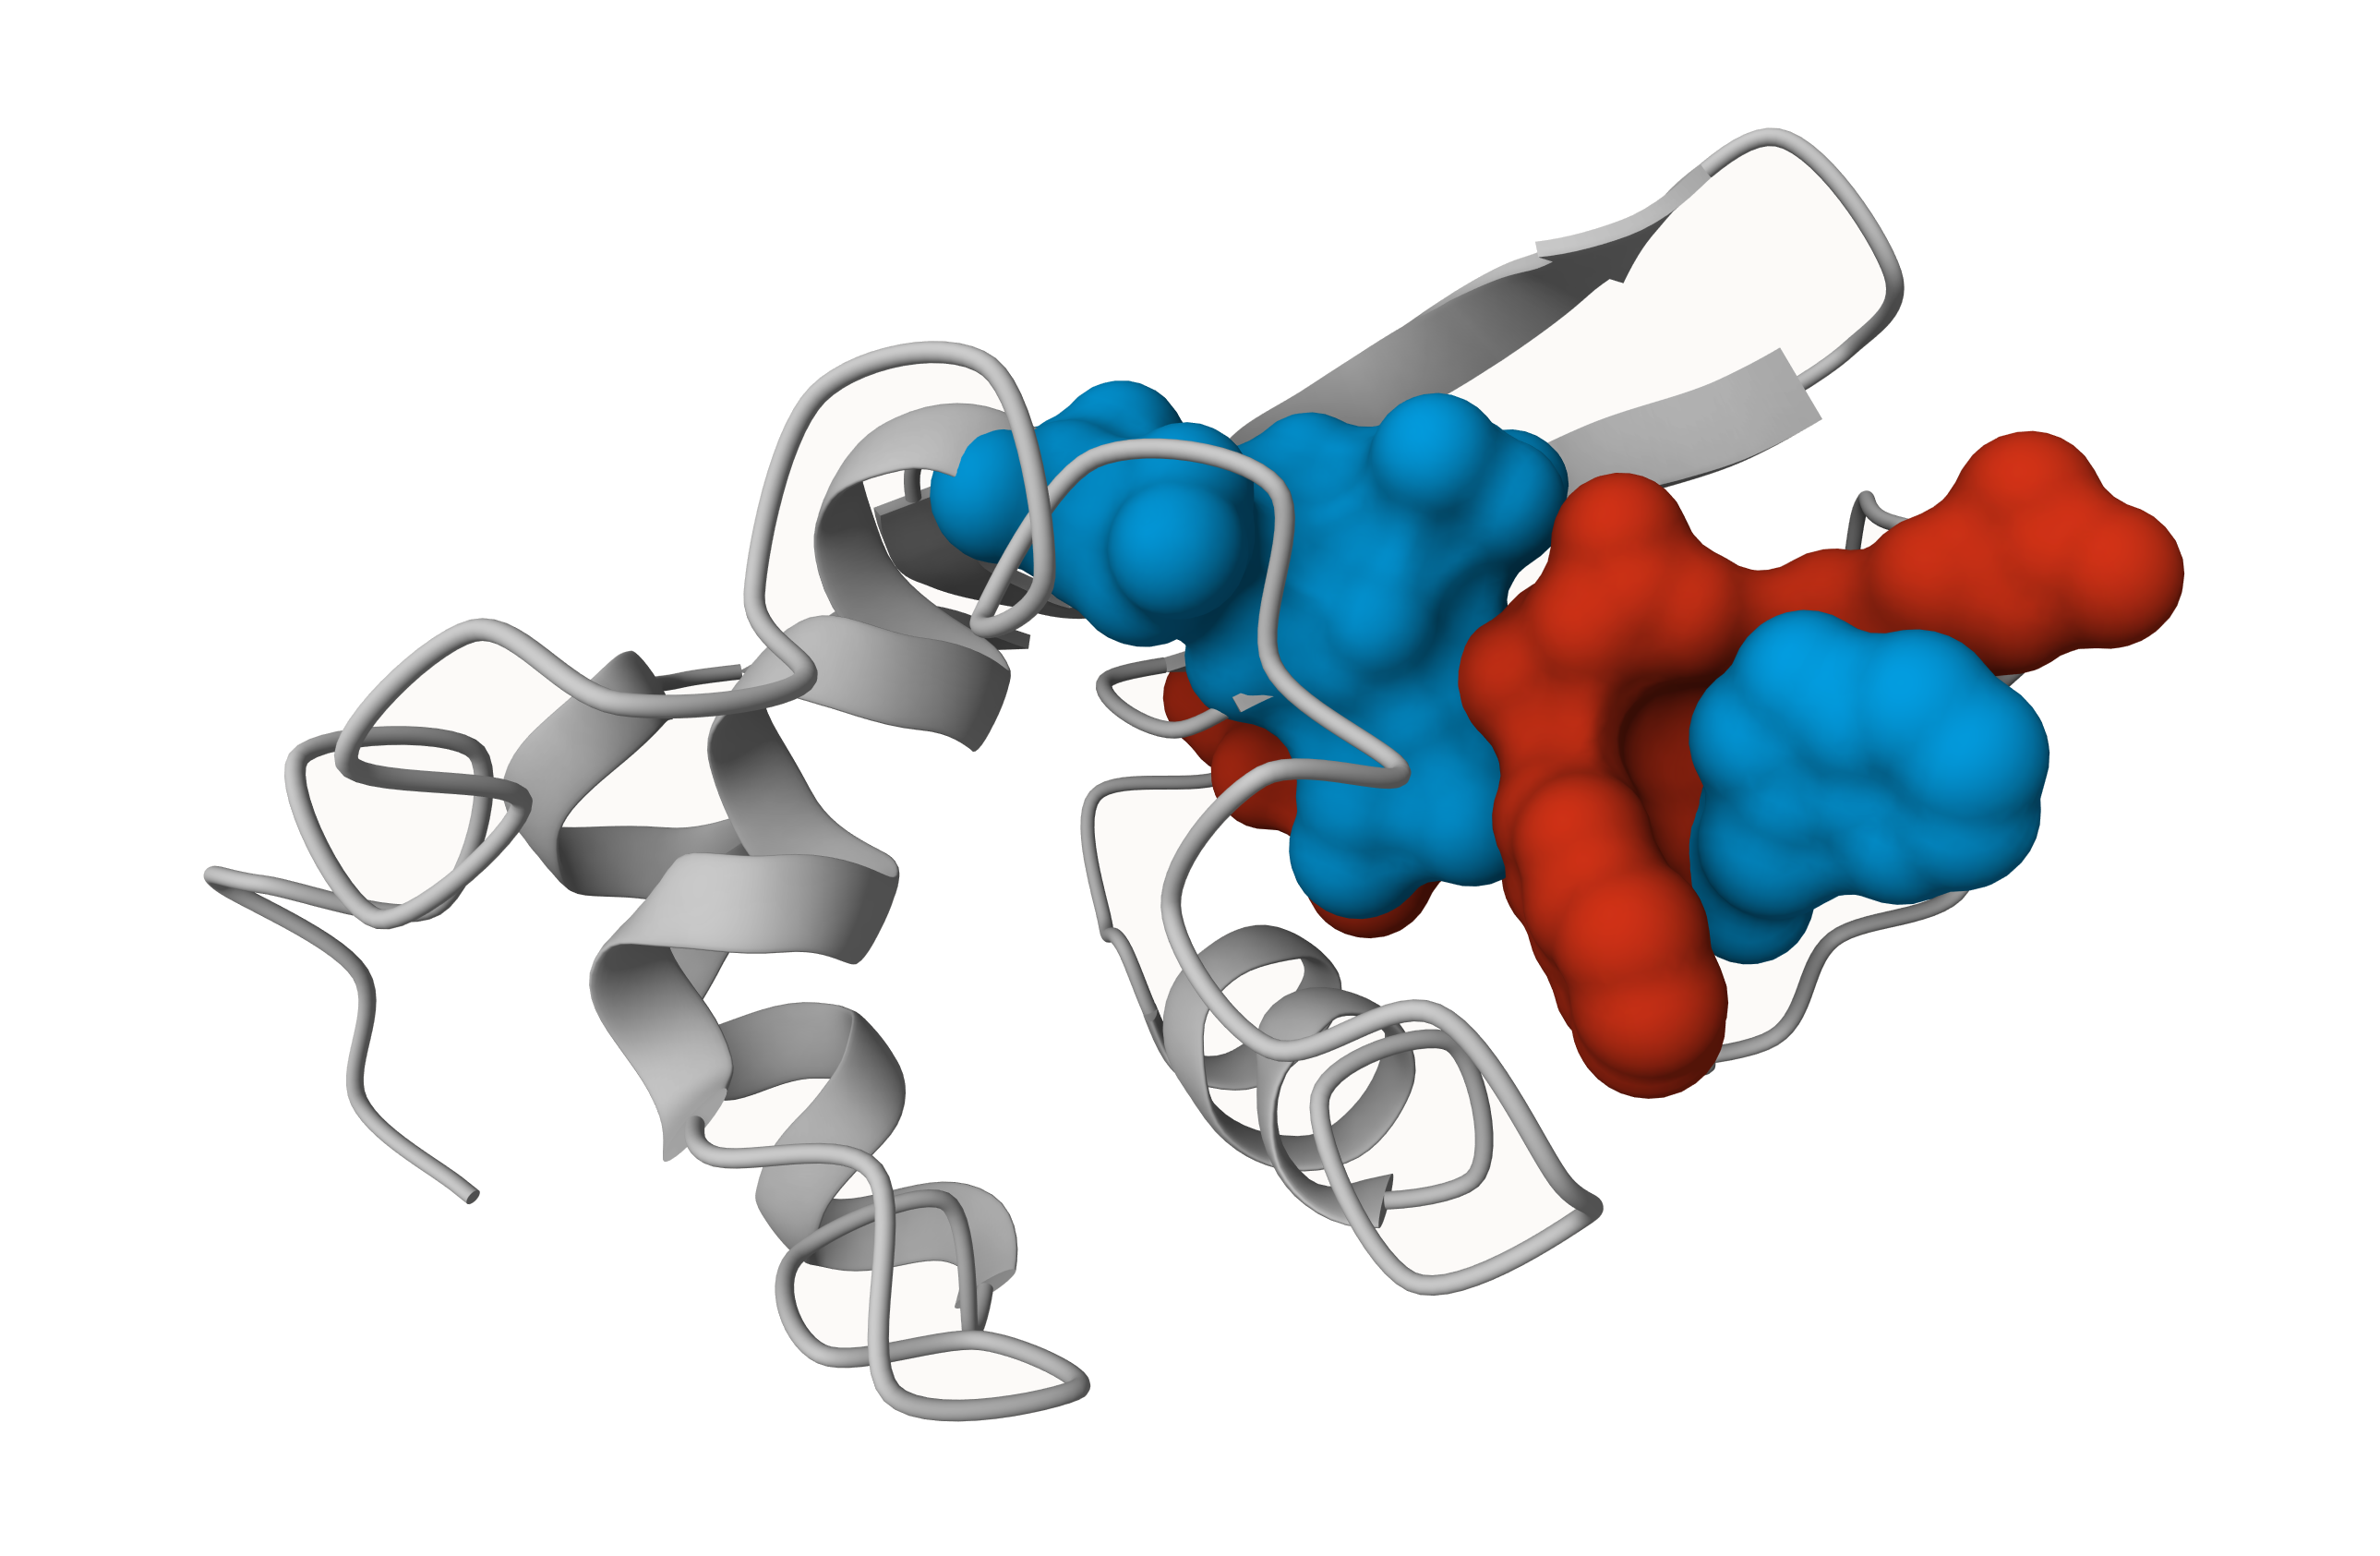
\includegraphics[width=\linewidth,height=0.8\textheight,keepaspectratio]{fig/smoothing-difference.png}
  \end{figure}
\end{frame}

\begin{frame}
  \frametitle{Evaluation on the CryptoBench dataset: Approach 2}

  \dots and it seems like the new model works!

  \begin{figure}
    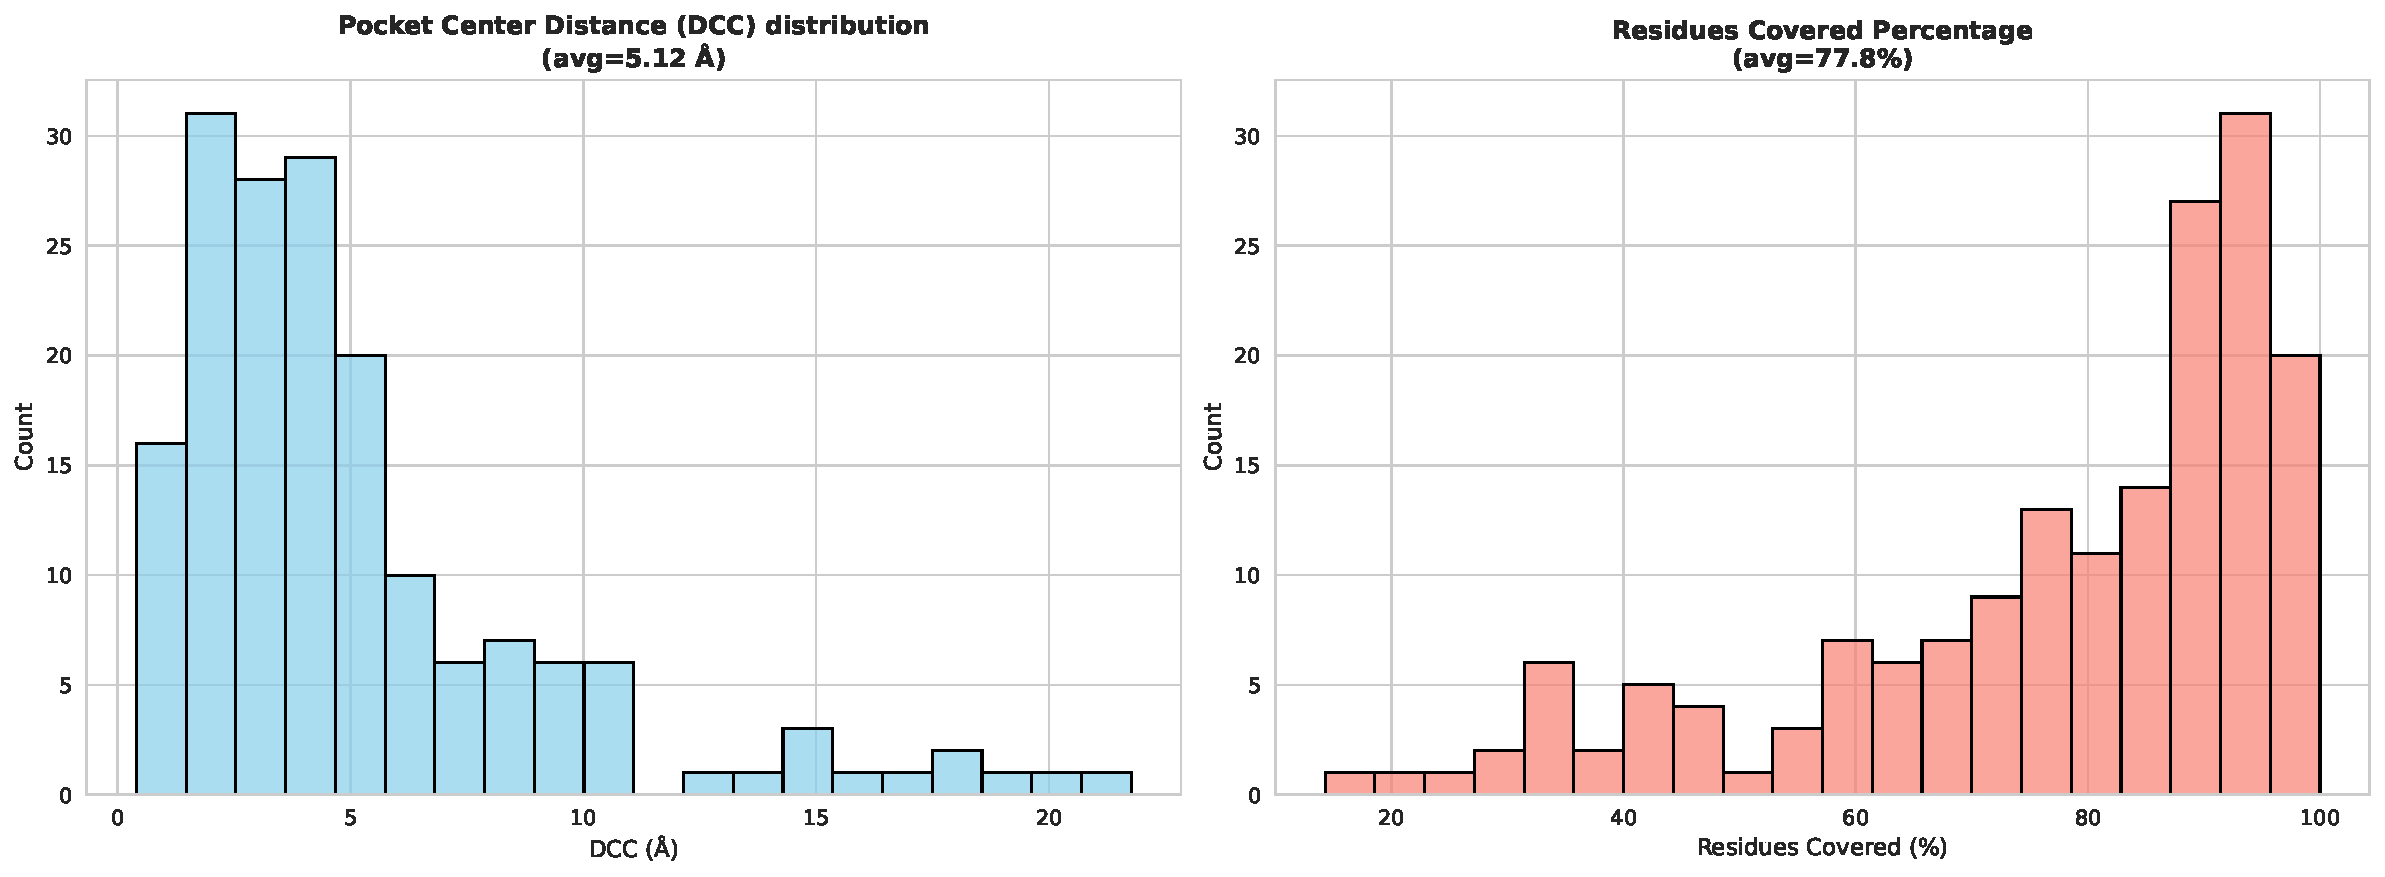
\includegraphics[width=\textwidth]{fig/smoothened-1.pdf}
  \end{figure}
\end{frame}

\section{Software}

\subsection{Architecture}

\begin{frame}
  \frametitle{Architecture}
  \begin{figure}
    \centering
    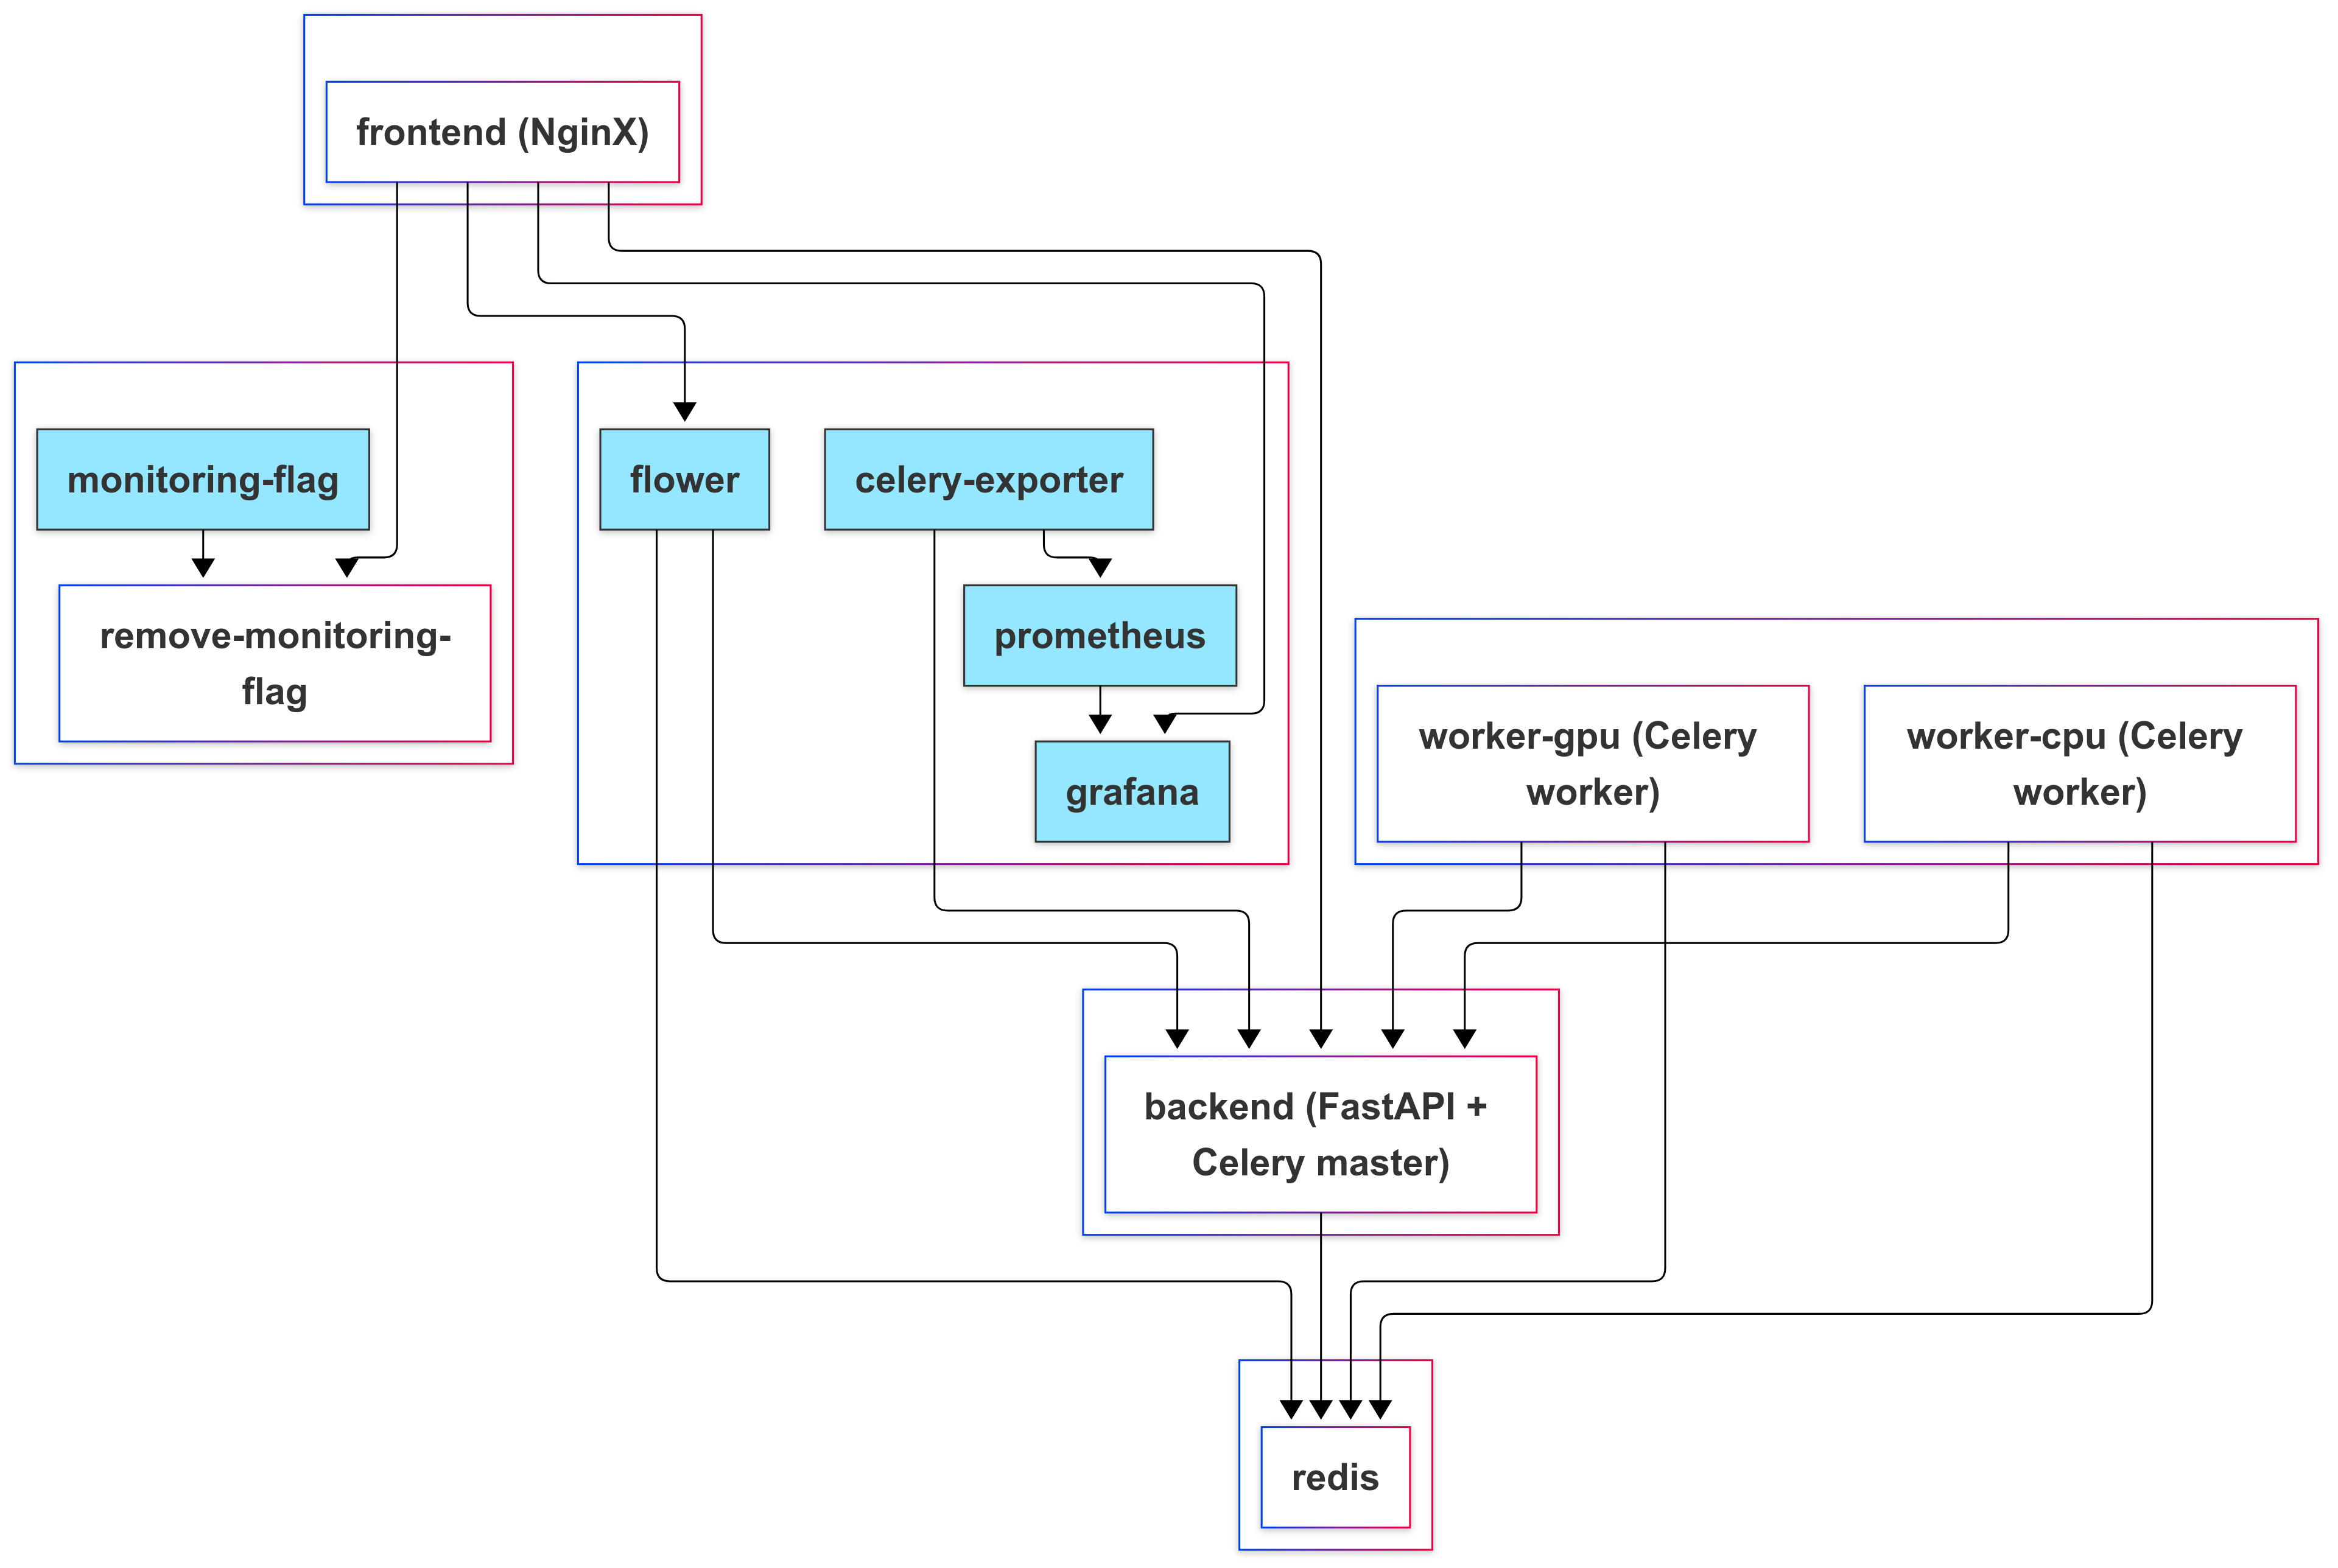
\includegraphics[width=\linewidth,height=0.8\textheight,keepaspectratio]{fig/architecture.png}
  \end{figure}
\end{frame}

\subsection{Technology Stack}

\begin{frame}
  \frametitle{Technology Stack}

  \begin{itemize}
    \item \textbf{Backend}: Python, notable libraries and tools: Celery (asynchronous tasks in Python), FastAPI, Flower, PyTorch, BioPython, Biotite, Scikit-Learn, MDAnalysis, Gemmi, Redis, uv
    \item \textbf{Frontend}: TypeScript, notable libraries, tools, and frameworks: React, NginX, Mol*, Bun, Vite
    \item \textbf{DevOps}: Docker (Docker Compose), GitHub Actions
  \end{itemize}

\end{frame}

\subsection{Screenshots}

\begin{frame}
  \begin{figure}
    \centering
    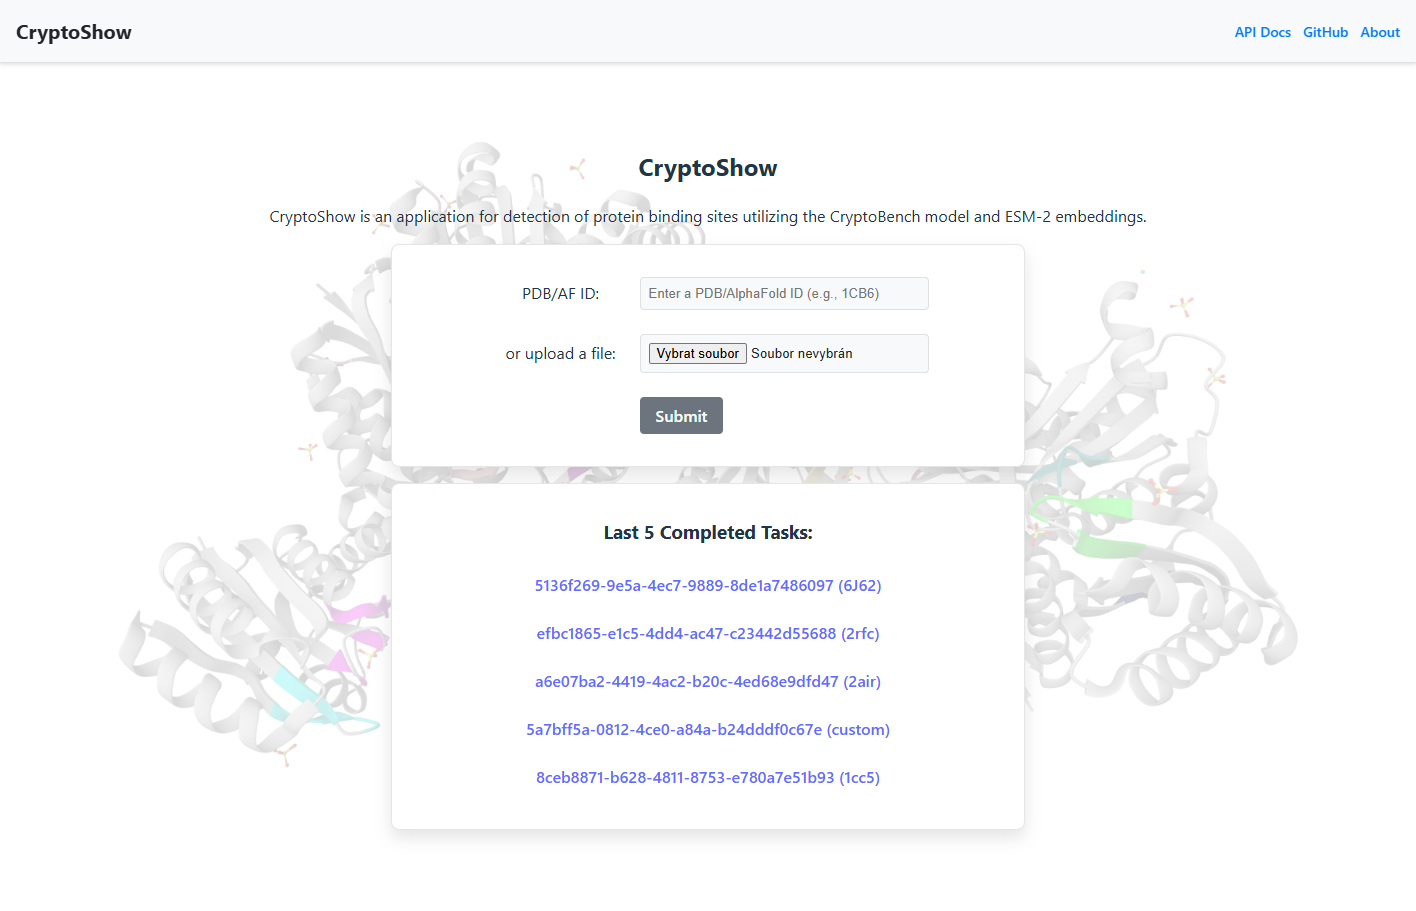
\includegraphics[width=\linewidth,height=\textheight,keepaspectratio]{fig/screen1.png}
  \end{figure}

\end{frame}

\begin{frame}
  \begin{figure}
    \centering
    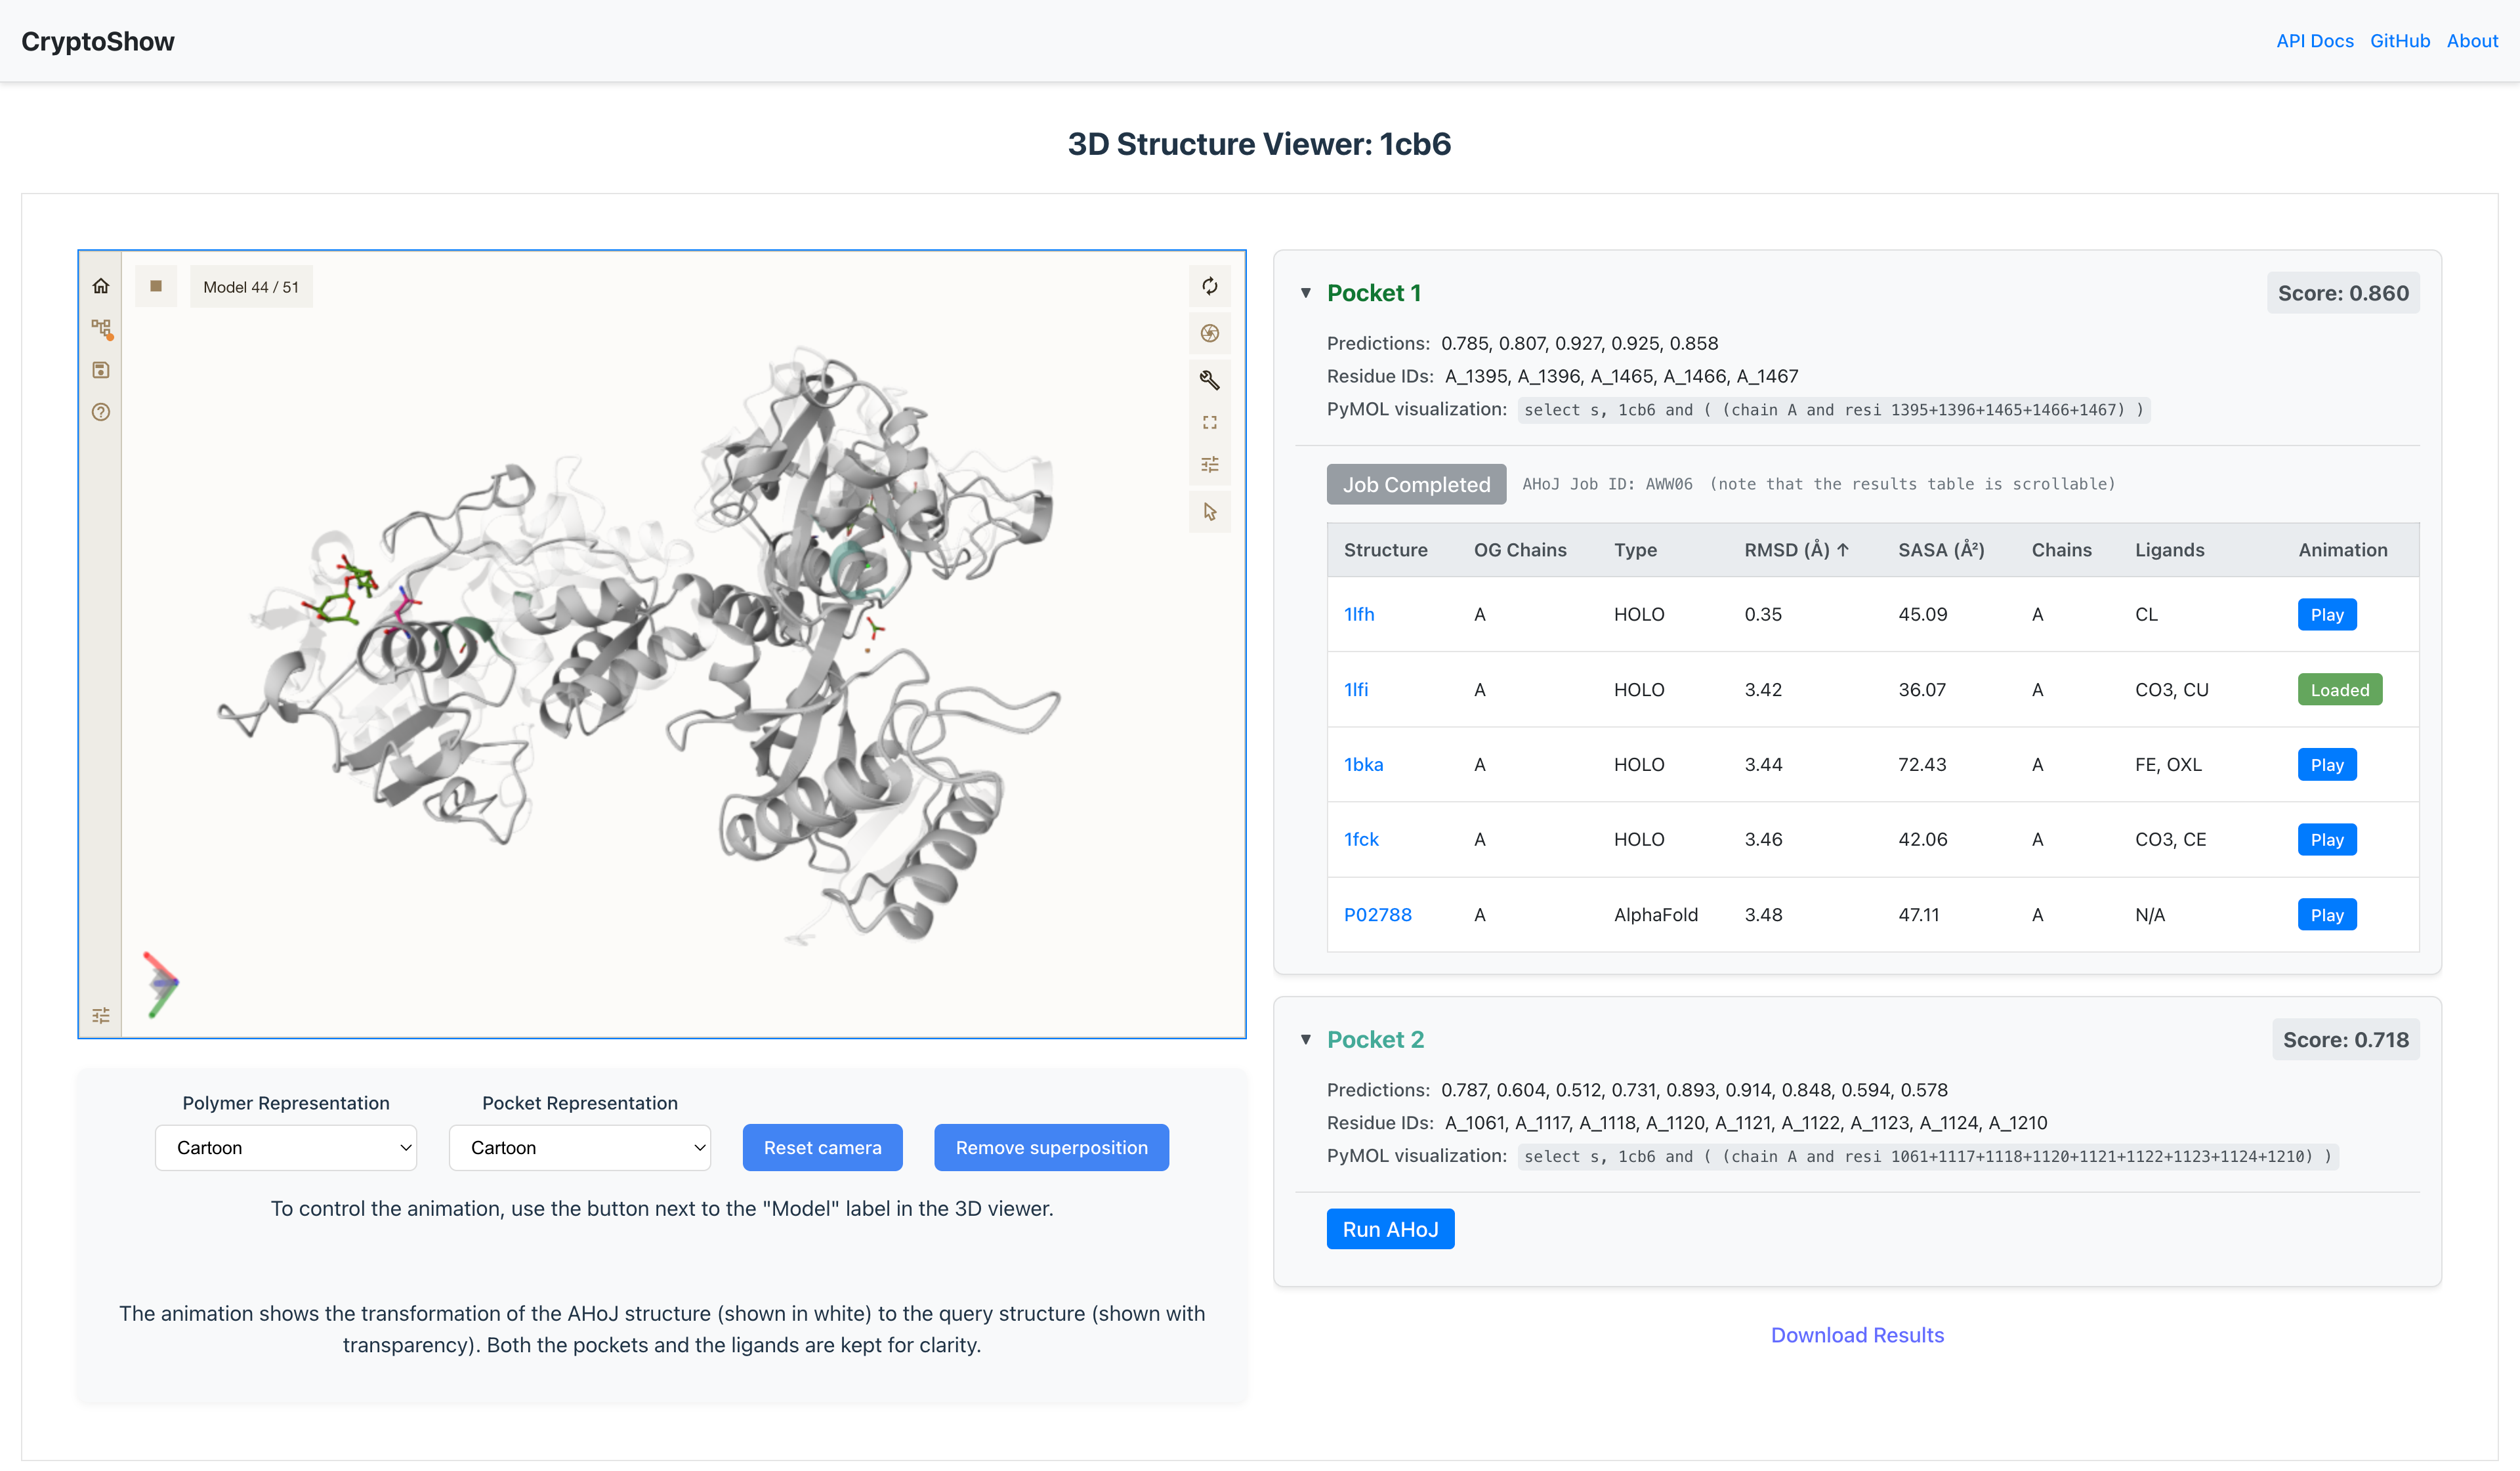
\includegraphics[width=\linewidth,height=\textheight,keepaspectratio]{fig/screen2.png}
  \end{figure}

\end{frame}

\begin{frame}
  \begin{figure}
    \centering
    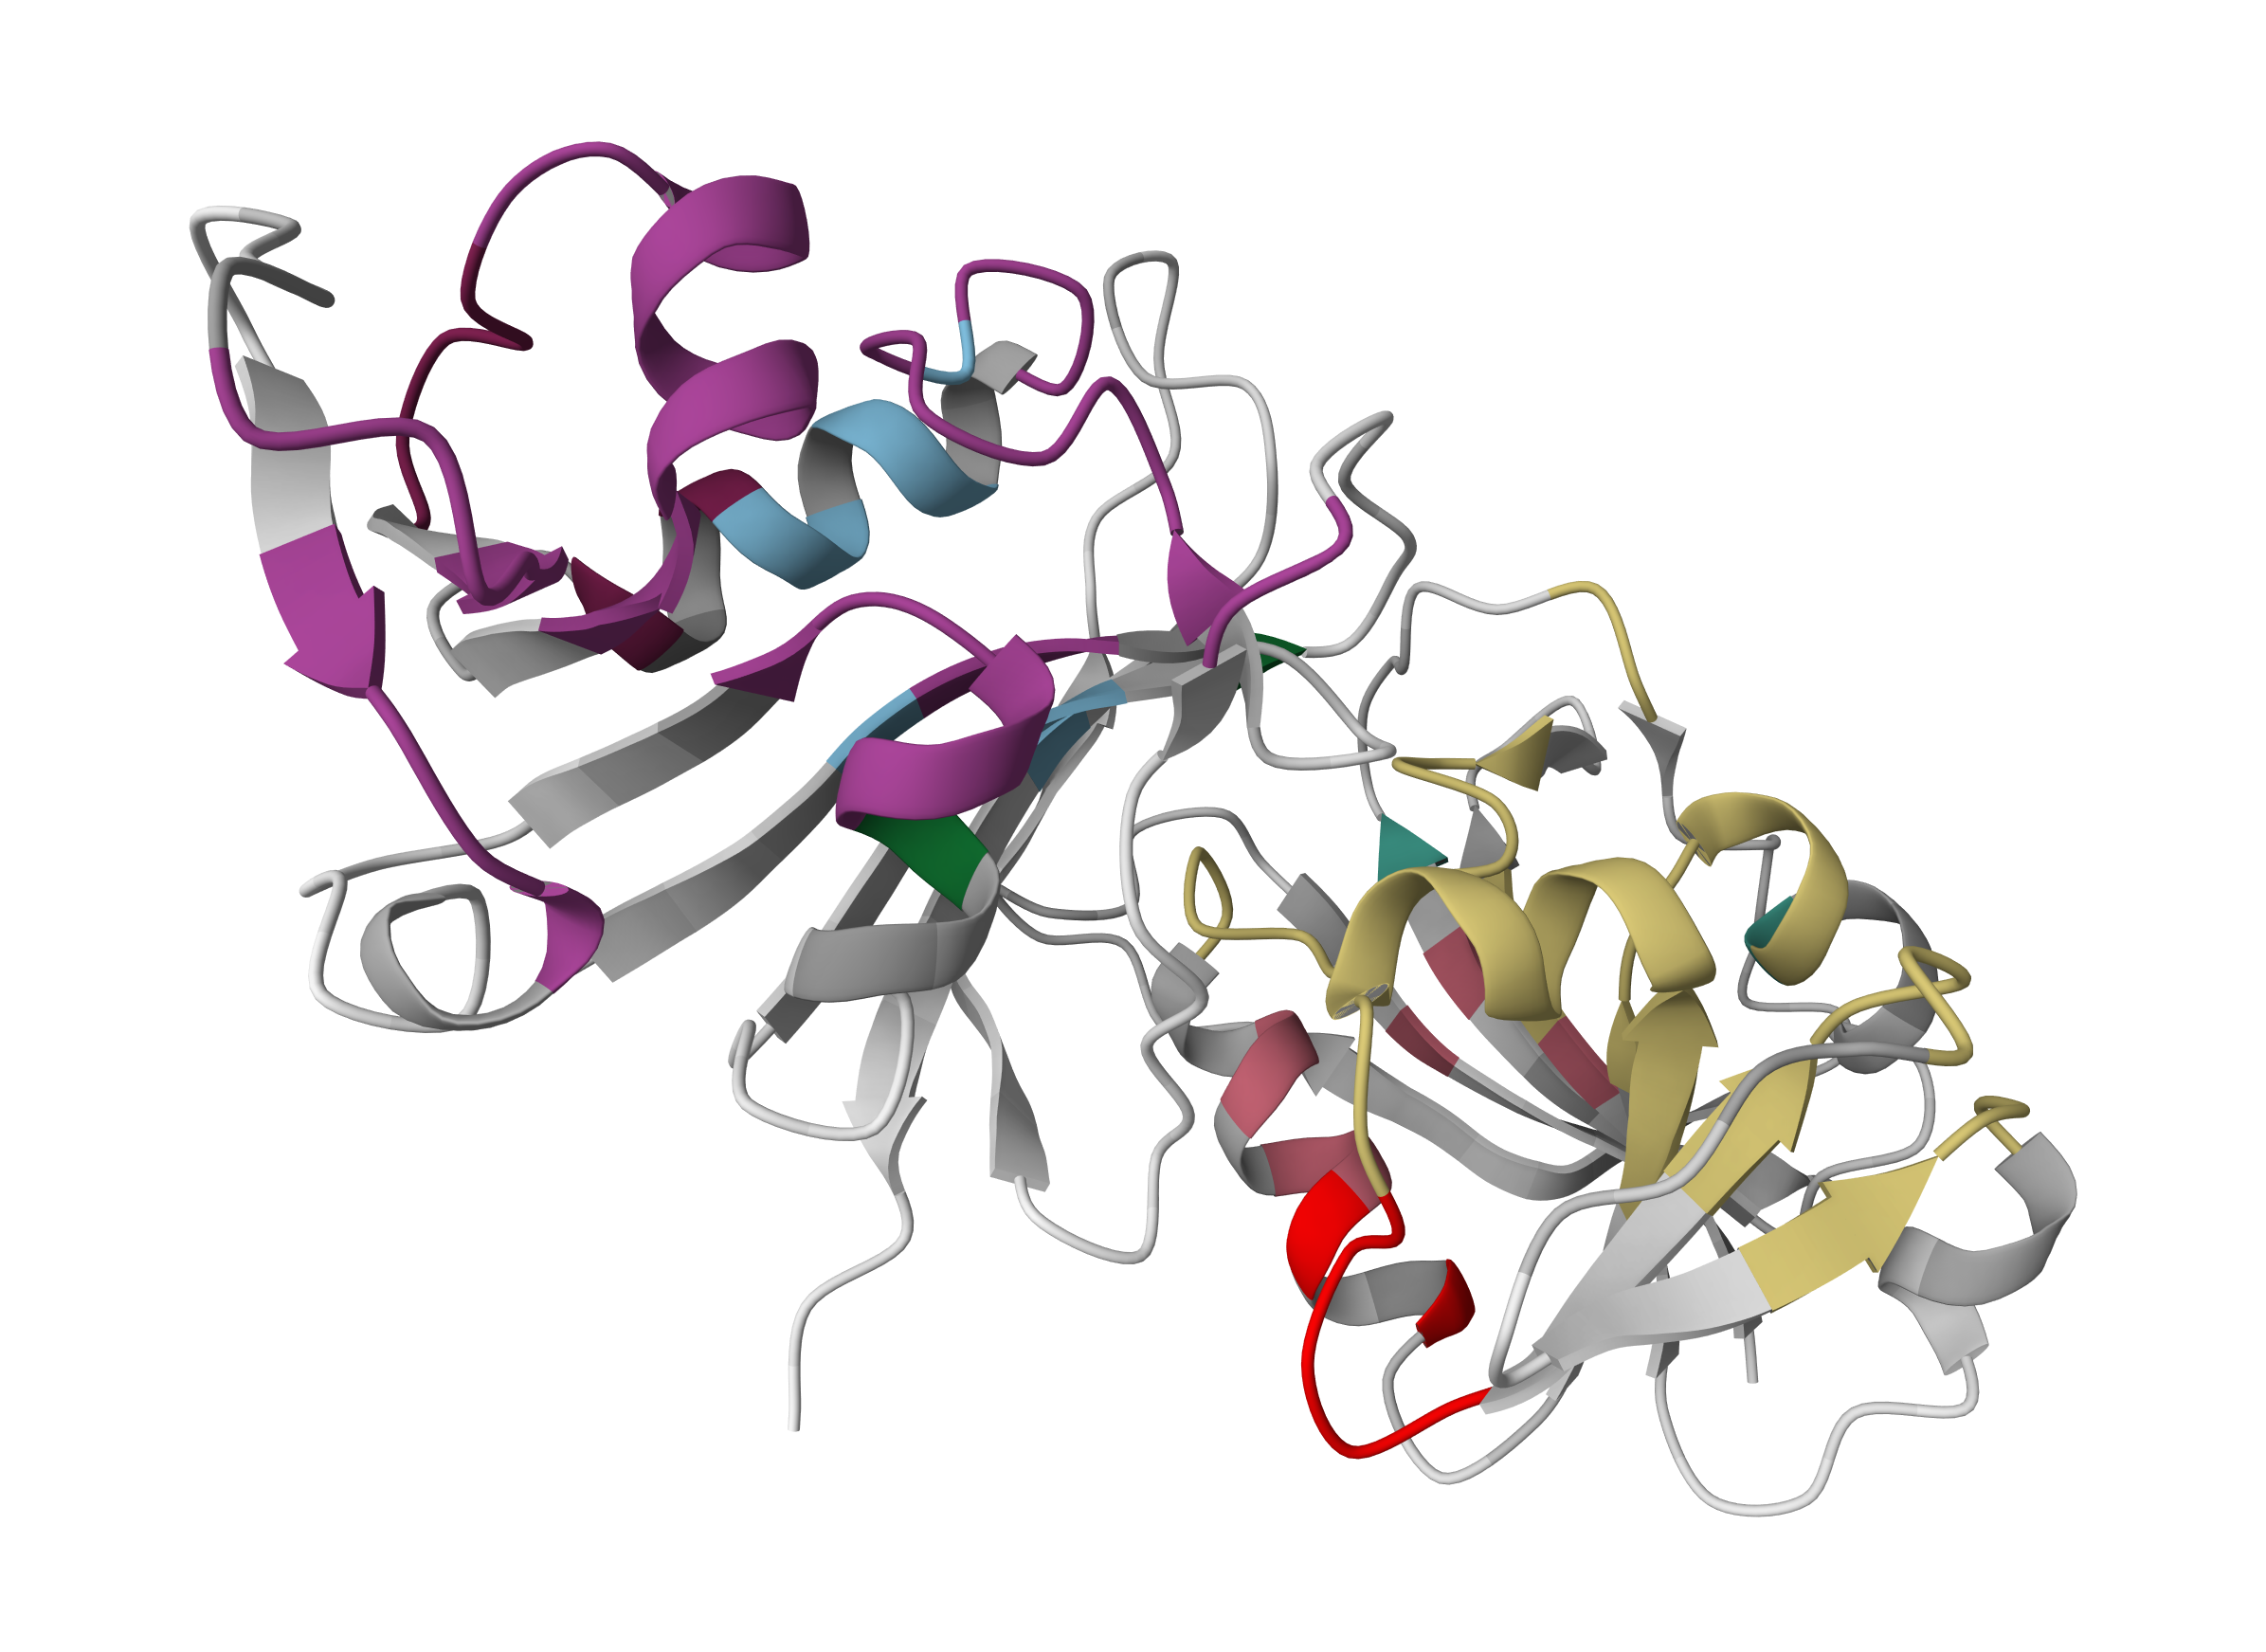
\includegraphics[width=\linewidth,height=\textheight,keepaspectratio]{fig/screen3.png}
  \end{figure}

\end{frame}

\begin{frame}
  \begin{figure}
    \centering
    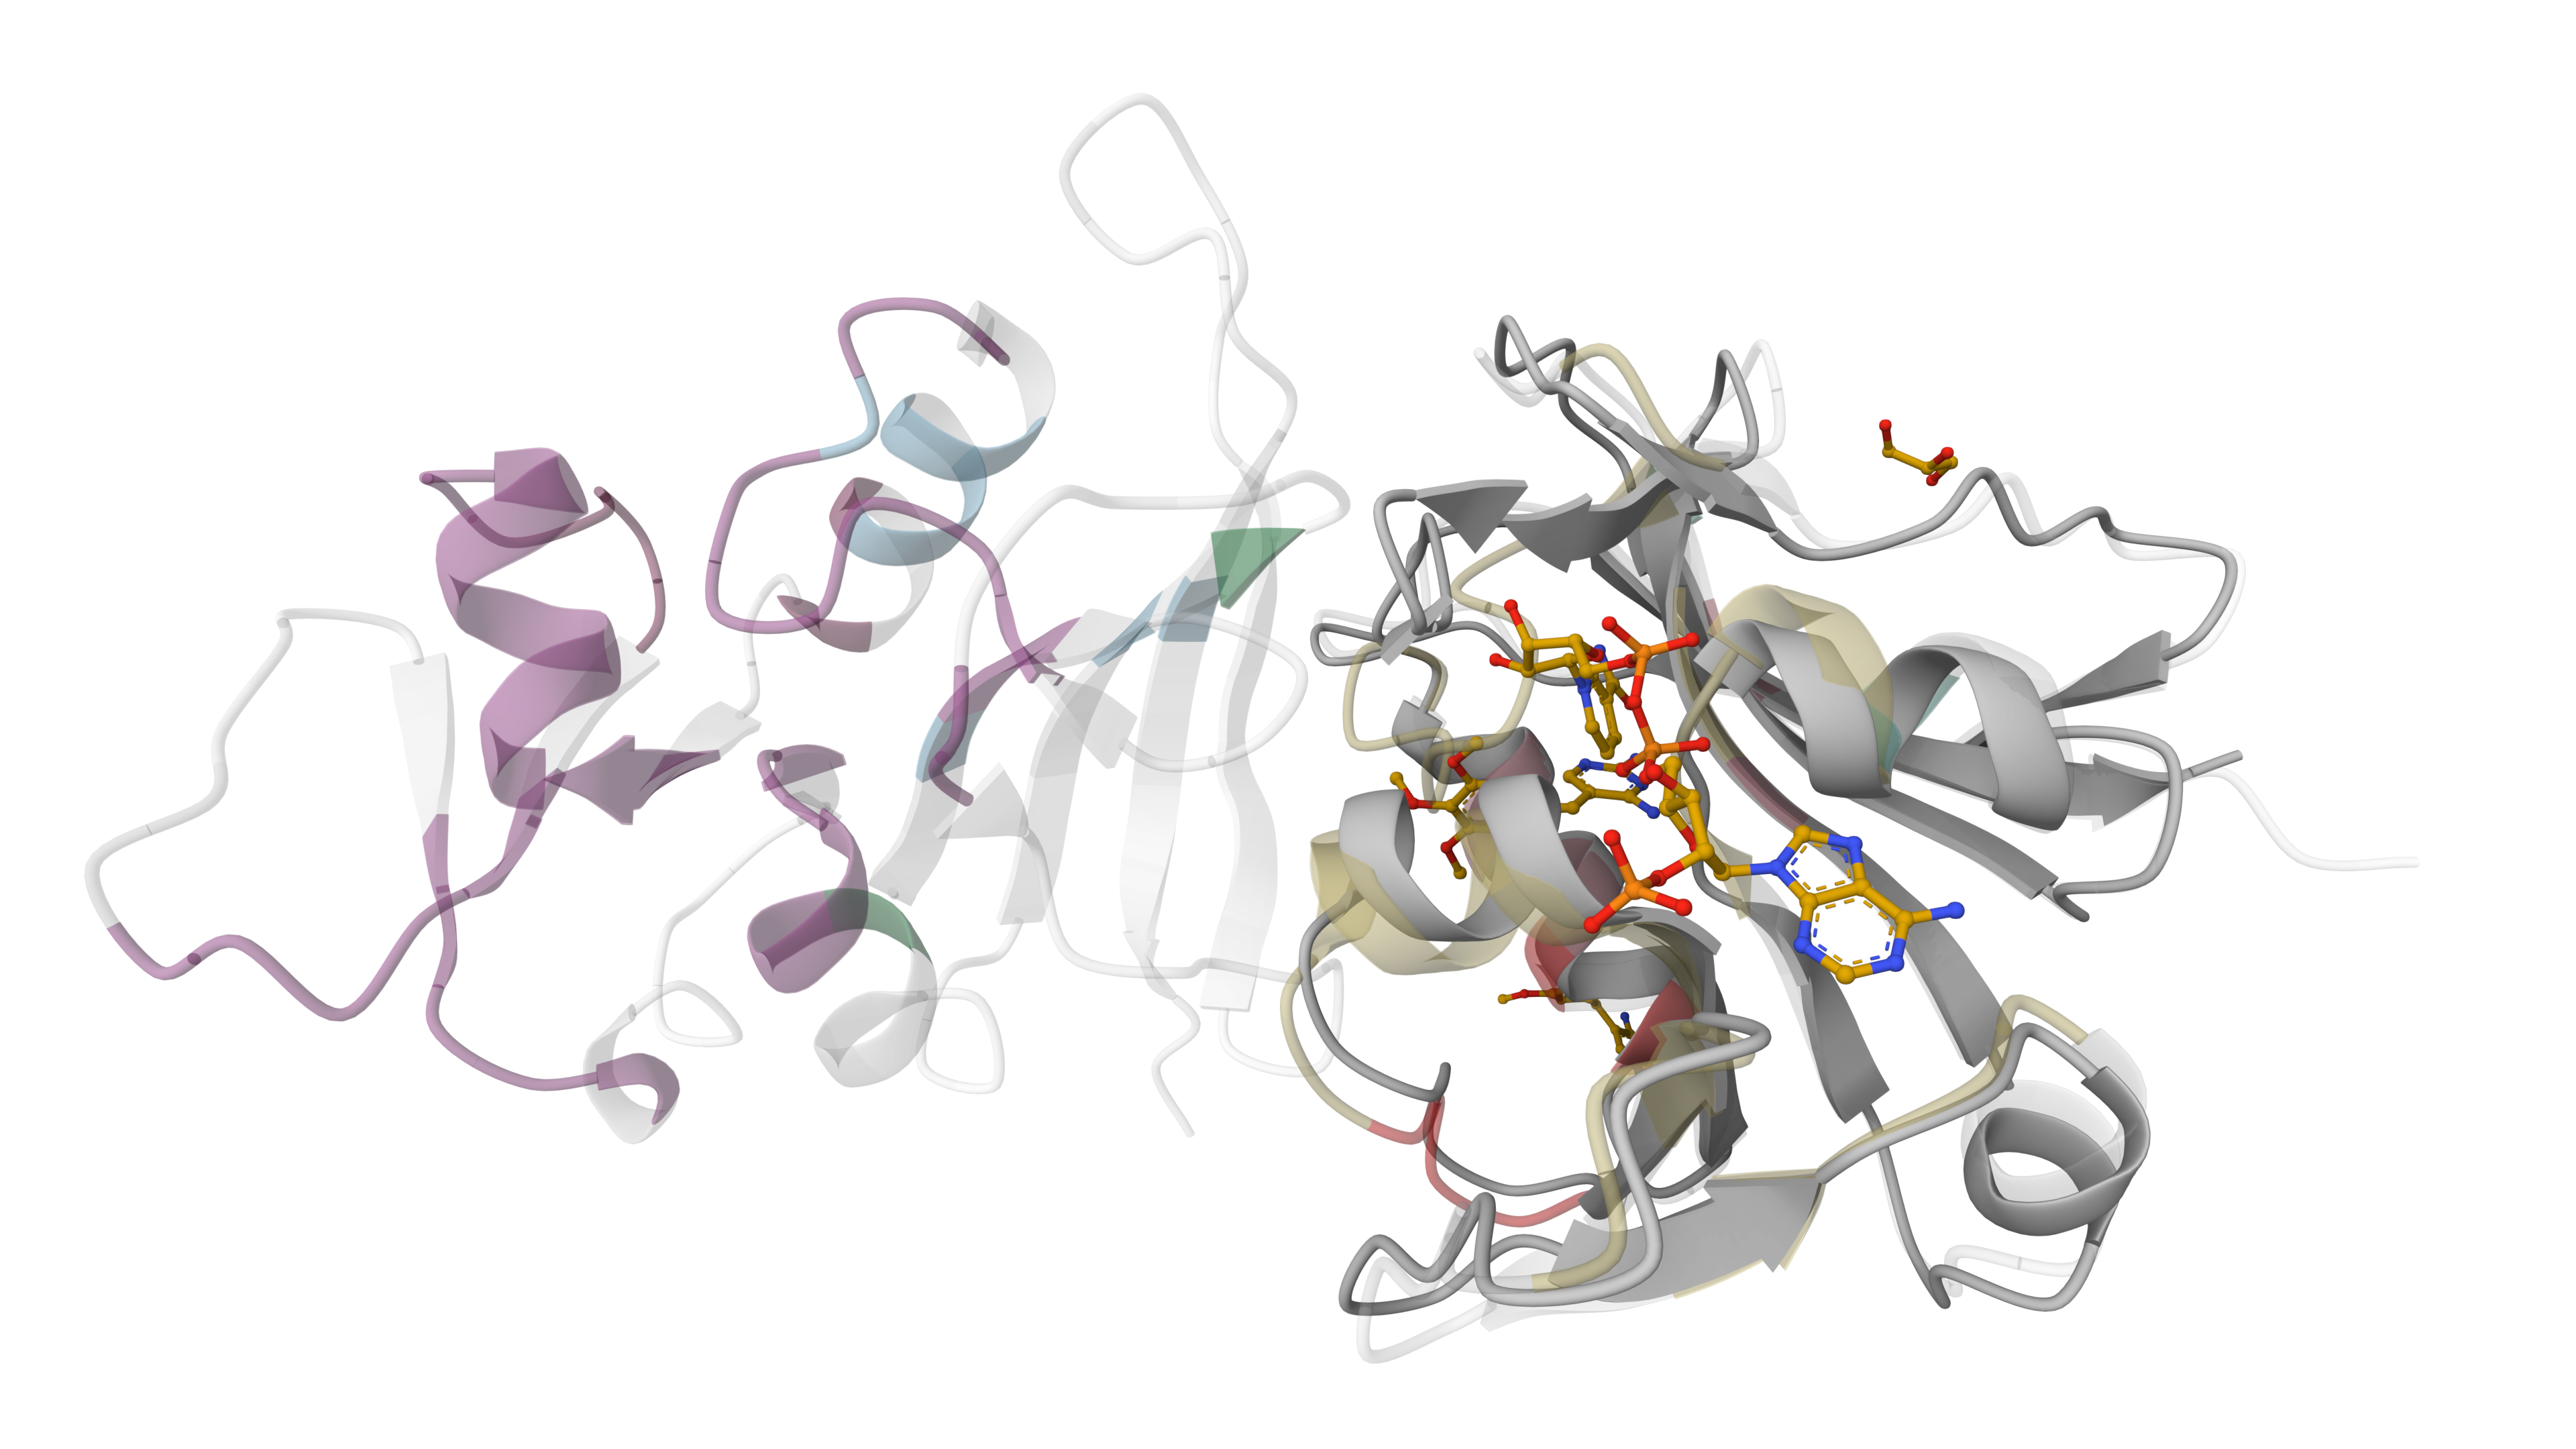
\includegraphics[width=\linewidth,height=\textheight,keepaspectratio]{fig/screen4.png}
  \end{figure}

\end{frame}

\begin{frame}[plain]
  \itmobackgroundsnakes{
    \vfill
    \Huge{The End}
    \vfill
  }
\end{frame}

\end{document}
